%TODO Checken, ob alle Fachwörter kursiv sind
\chapter{Sicherheit in Datenbanken}
%TODO Formulierungen anpassen
Datenbanken stellen heutzutage allgegenwärtige Systeme dar. Die persistente Datenhaltung sowie die effiziente Möglichkeit zur Bereitstellung angefragter Datenmengen machen sie unverzichtbar in Infrastrukturen, welche auf Grundlage größerer Informationsbestände arbeiten. Maßnahmen in Bezug auf die Sicherheit jener Systeme bezogen sich klassischerweise auf den Schutz vor unberechtigtem Zugriff auf entsprechende Datenbankserver bzw. das Absichern vor unerlaubter Modifikation des Datenbestandes, jeweils von außen \cite{BSI1}. Durch den stärkeren Einsatz von Datenbanklösungen in nicht vertraulichen Umgebungen, wie etwa in der Cloud, ergeben sich neue Herausforderungen in Bezug auf den Schutz der Informationen. In diesem Kapitel soll ein Überblick über jene Sicherheitsaspekte gegeben werden. Neben der Darstellung verschiedener Lösungskonzepte dieser Problematik aus anderen Publikationen wird ein besonderer Fokus auf die Funktionsweise von Intel SGX, als den später zu untersuchenden Ansatz, gelegt. Im Grundlagenteil werden zunächst eine erweitere Einführung in die Datenbanksicherheit im Kontext der Arbeit gegeben und relevante Begriffe erklärt. Nachfolgend stehen verwandte Arbeiten im Vordergrund. Das Konzept und der Aufbau von Intel SGX werden im letzten Abschnitt untersucht.

\section{Grundlagen}
Um grundsätzlich ein System in Bezug auf seine (Informations-)sicherheit zu betrachten, ist es notwendig, dieses auf die Einhaltung gewisser Merkmale hin zu charakterisieren. Diese als Schutzziele bezeichneten Eigenschaften fallen je nach Kontext anders aus. Im Allgemeinen bestehen sie jedoch den drei Begriffen Vertraulichkeit, Integrität und Verfügbarkeit:

\paragraph{Vertraulichkeit}
Als Vertraulichkeit bezeichnet man die Eigenschaft, dass Informationen in einem System nur denjenigen Subjekten zur Verfügung steht, welche dazu berechtigt sind.

\paragraph{Integrität}
Integrität liegt vor, wenn jegliche Modifikation einer Datenmenge zu jeder Zeit erkannt werden kann.

\paragraph{Verfügbarkeit}
Ein System besitzt Verfügbarkeit, wenn es fortlaufend unter korrekter Funktionsweise verfügbar ist.

\paragraph{}
Im Kontext dieser Arbeit wird konkret ein Datenbanksystem betrachtet, welches sich zwar unter der Kontrolle einer berechtigten Partei, jedoch in einem nicht vertrauenswürdigen Umfeld befindet. Ein potenzieller Angreifer ist in diesem Fall zum einen ein böswilliger oder neugieriger Administrator des Drittsystems. Auf der anderen Seite ist es stets möglich, dass sich eine Person unbemerkt physischen Zugriff auf das System verschaffen hat, welches sich schließlich außerhalb des eigenen Zuständigkeitsbereichs befindet \cite{Popa2012}. Da es im Kontext dieser Arbeit hauptsächlich um die Vertraulichkeit in Bezug auf sensitive Daten geht, werden Integrität und Verfügbarkeit im Folgenden stets außer Acht gelassen. 

Erreicht wird Vertraulichkeit in der Regel durch den Einsatz eines kryptographischen Verfahrens, welches die Ver- und Entschlüsselung von Daten erlaubt. Einem Angreifer ist es ohne das Wissen über den Schlüssel nicht möglich, Informationen aus den verschlüsselten Daten zu gewinnen, zumindest falls es sich um ein kryptographisch sicheres Verfahren handelt. Während jene Schemata in vielen Kontexten, wie etwa Kommunikationsprotokollen, ihren Einsatz finden, ergeben sich besondere Bedingungen bei der Verwendung innerhalb eines Datenbanksystems. Eine reine Speicherung von Daten auf verschlüsselter Basis stellt im Grunde kein Problem dar. Jedoch ist es früher oder später nötig, Berechnungen auf dem Datenbestand durchzuführen, um beispielsweise die Ergebnismenge zu einer Datenbankanfrage (Query) zu bestimmen. Da übliche Verschlüsselungsverfahren keine Berechnungen auf Schlüsseltexten erlauben, ist eine temporäre Entschlüsselung notwendig. Diese kann unter Gewährleistung der Vertraulichkeit nicht auf dem Server selbst ausgeführt werden, da sonst Klartextdaten im Speicher vorhanden wären. Eine reine Entschlüsselung und Verarbeitung auf Seiten des Clients ist auf der anderen Seite hoch unpraktikabel, wenn es sich um große Datenbestände handelt \cite{Popa2012}.

\section{Verwandte Arbeiten}
%TODO Etwas Kürzen
Auf dem Gebiet der sicheren Datenhaltung und -verarbeitung gab es in der Vergangenheit bereits viele vielversprechende Lösungsansätze. In diesem Kapitel wird ein Überblick über entsprechende Arbeiten gegeben. Die größten Vertreter werden zudem etwas genauer auf ihre Vor- und Nachteile untersucht. Hierbei sind die Hauptmerkmale vor allem die zur Verfügung gestellte Sicherheit, unter dem kryptographischen Gesichtspunkt und auch der Möglichkeit zur Anpassbarkeit jener. Darüber hinaus stellt sich auch die Frage, inwieweit die Funktionalität des Datenbanksystems beeinflusst wird. Etwa, ob es eine Einschränkung der Datenbankschnittstelle gibt, z.B. in Bezug auf die zur Verfügung stehenden Anfragen, oder ob starke Kompromisse auf leistungstechnischer Ebene eingegangen werden müssen.

Ein grundlegender Ansatz, den alle betrachteten Arbeiten gemeinsam haben, ist die Auslagerung und Verschlüsselung der zugrundeliegenden Datenbank. Entsprechend findet meist eine klare Trennung zwischen der reinen Datenspeicherung und der Verarbeitung statt, wobei letztere stets eine unabhängig betrachtete Komponente darstellt. Es lassen sich dennoch zwei Kategorien von Ansätzen festmachen. Zum Ersten ist dies ein rein auf dem Verschlüsselungsverfahren beruhendes Prinzip. Die Daten werden hierbei mit einem bestimmten Schema verschlüsselt, so dass weiterhin eine Verarbeitung stattfinden kann, ohne auf eine Repräsentation in Klartext zugreifen zu müssen. Der zweite Ansatz beruht auf die Einbeziehung von vertraulichen Hardwarekomponenten in den Berechnungsprozess. Diese agieren als sogenannte Vertrauensbereiche und erlauben ein Arbeiten auf den Klartextdaten, ohne dass ein potenzieller Angreifer einen Einblick in diese bekommen kann. Zusammen mit der Software, die innerhalb von ihnen ausgeführt wird, bilden diese Bereiche die sogenannte Trusted Computing Base (TCB) des Systems und sollten frei von Fehlern sein, welche mögliche Sicherheitslücken eröffnen können. Mit der Zeit erfolgte zusätzlich eine Integration von Methoden der ersten Herangehensweise in die Verarbeitung innerhalb der sicheren Bereiche, um die Stärken beider Konzepte zu kombinieren.

Zunächst wird in diesem Kapitel auf Arbeiten aus der ersten Kategorie eingegangen. Der bekannteste Vertreter ist hierbei CryptDB. In seinem Bereich bildet es den Grundstein für die weiteren hier aufgeführten Arbeiten und wird etwas genauer behandelt. Basierend auf Vertrauensbereichen sind sehr vielfältige Arbeiten entstanden. Betrachtet werden hier vor allem TrustedDB und Cipherbase. In Abbildung \ref{fig:timeline} ist eine einfache zeitliche Einordnung der verschiedenen Arbeiten zu sehen.

\begin{figure}
	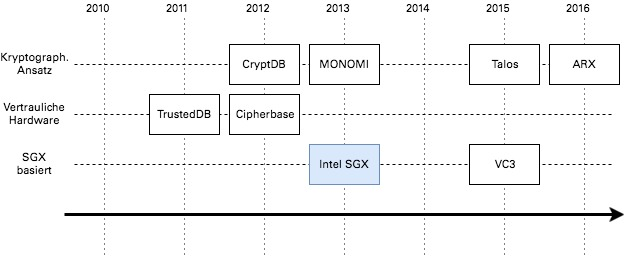
\includegraphics[width=0.9\linewidth]{img/RelatedWorkTimeline.pdf}
	\centering
	\caption{Zeitliche Einordnung verwandter Arbeiten nach Kategorie}
	\label{fig:timeline}
\end{figure}

Genau wie die meisten anderen Systeme, wurde CryptDB \cite{Popa2011}\cite{Popa2012} für die Arbeit auf relationalen SQL Datenbanken entworfen. Der Kern von CryptDBs Architektur ist ein Proxy Server, der sich zwischen dem Anwendungs- und  Datenbankserver befindet. Sobald eine Anfrage an die verschlüsselte Datenbank gestellt wird oder eine Antwort zurückkommt, verlaufen diese zunächst über jenen Proxy, der im Normalfall ebenfalls auf dem Anwendungsserver läuft. Ein vereinfachtes Schema der Architektur ist in Abbildung \ref{fig:cryptdb} zu sehen. CryptDB nutzt den Aufbau von SQL Anfragen aus mehreren einfachen Operationen wie Joins, Gleichheitsprüfungen oder Ordnungen auf Werten aus, um diese direkt auf den verschlüsselten Daten durchführen zu können. Das entsprechend eingesetzte Schema wird als \textit{SQL aware encryption} bezeichnet. Es definiert die kryptographischen Methoden, welche für die Ausführung einer bestimmten Operation notwendig sind. Ist es beispielsweise nur nötig, eine Selektion mit Gleichheitsbedingung durchzuführen, so genügt ein deterministisches Verschlüsselungsverfahren, welches stets den gleichen Schlüsseltext für einen gegebenen Klartext produziert. Will man allerdings den minimalen oder maximalen Wert, bzw. eine geordnete Ergebnismenge erhalten, so ist es nötig ein schwächeres Verfahren einzusetzen, welche die Ordnung von Klartextwerten durch das Verschlüsseln erhält, sogenannte \textit{Order Preserving Encryption}. Um eine möglichst große SQL Funktionalität bereitzustellen und dennoch das höchstmögliche Maß an Vertraulichkeit, setzt CryptDB auf ein sogenanntes \textit{Onion Scheme}. Jeder Wert ist in mehreren Schichten verschlüsselt, wobei die gegebene Sicherheit mit jeder Schicht zunimmt, ebenso nehmen die möglichen Operationen ab. Entschlüsselt wird dann nur bis zu der Schicht, welche für die aktuellen Berechnungen nötig ist. Die benutzten Schlüssel liegen je Nutzer auf dem Anwendungsserver. Der Proxy selbst besitzt jedoch einen Masterkey, um Anfragen umschreiben zu können. Da jeder Benutzer des Systems über einen individuellen Schlüssel verfügt, ist es möglich, gewisse Daten für einzelne Nutzer freizugeben oder zu verstecken. Hierfür hält der Proxy ein spezielles Schema. Die Datenverarbeitung selbst erfolgt durch UDFs (User Defined Functions) auf dem Datenbankserver, nachdem der Proxy die eingehende Anfrage umgeschrieben hat. Infolge der Auslieferung von den verschlüsselten Ergebnisdaten an den Proxy, kann dieser die Entschlüsselung vornehmen und sie dem Anwendungsserver liefern.

Trotz der zusätzlichen Bearbeitung im Proxy, hat CryptDB einen relativ geringen Performance Overhead im Vergleich zum herkömmlichen unsicheren Ablauf \cite{Popa2012}. Die Nachteile des Verfahrens liegen allerdings in den eingeschränkten Möglichkeiten an SQL Anfragen, sowie den fehlenden Konfigurationsmöglichkeiten in Bezug auf die gewünschte Sicherheit. Die absichtliche Nutzung schwächerer Verschlüsselungsverfahren wie OPE, erleichtern einem Angreifer, Aussagen über die Schlüsseltexte zu treffen \cite{Poddar2016}.

Zwei Jahre nach der Veröffentlichung von CryptDB folgte mit MONOMI \cite{Tu2013} ein nachfolgendes System, welches auf dem Verschlüsselungsschema aufbaute, jedoch für den Anwendungsfall von analytischen Workloads angepasst wurde. Diese unterscheiden sich größtenteils dadurch, dass viel größere Datenmengen auf komplexe Art verarbeitet werden. Dies bringt auf einer komplett verschlüsselten Datenbank viele Probleme mit sich, unter anderem, wie jene komplexen Anfragen effizient auf verschlüsselten Daten ausgeführt werden können. MONOMI verteilt hierzu die Ausführung der Anfragen auf Server und Client. Bei Letzterem können so etwa letzte Verarbeitungsschritte ausgeführt werden, nachdem die Daten schon unverschlüsselt sind, während jene auf dem Server mit den verschlüsselten Daten deutlich aufwendiger wären. MONOMI bringt zudem noch weitere Leistungsoptimierungen mit und schneidet bei großen Benchmarks sowohl in Bezug auf Speicherbedarf und Leistung deutlich besser ab als CryptDB \cite{Tu2013}.

An dieser Stelle muss auch kurz Talos \cite{Shafagh2015} erwähnt werden. Das 2015 beschriebene System baut ebenso auf CryptDB auf, vereinfacht und optimiert das Konzept jedoch für den Einsatz im Internet of Things. Die eingesetzten kryptographischen Algorithmen, z.B. für OPE werden durch leistungsfähigere Varianten ersetzt und erlauben die Ausführung auf Systemen mit beschränktem Energiebudget und Speicherplatz.

Der letzte hier genannte Vertreter in der Kategorie ausschließlich auf Kryptographie beruhender Systeme ist Arx \cite{Poddar2016}. Es handelt sich dabei um einen ganz offiziellen Nachfolger von CryptDB, der 2016 veröffentlicht wurde. Diesmal verfolgte man eine neue Herangehensweise, indem man die Berechnungen nicht auf den eingesetzten Verschlüsselungsverfahren aufsetzt, sondern in spezielle Datenstrukturen. Dies erlaubt es, komplett unabhängig vom Verschlüsselungsverfahren zu sein, was wiederum erlaubt, ausschließlich starke und anerkannte Standardverfahren wie AES zu nutzen. Ermöglicht wird dies durch die Nutzung von speziellen Datenbankindizes, welche speziell zum Traversieren verschlüsselter Daten entworfen wurden und die Sicherheit dahingehend gewähren, dass die Knoten in den Indexstrukturen nach jeder Benutzung zerstört und entsprechend erneuert werden müssen.

\begin{figure}
	\includegraphics[width=0.9\linewidth]{img/RelatedWorkCryptDB.pdf}
	\centering
	\caption{Architektur von CryptDB}
	\label{fig:cryptdb}
\end{figure}

Auf Seiten der Verfahren, welche anstatt der reinen Arbeit auf verschlüsselten Daten vertrauliche Hardwarekomponenten nutzen, soll zunächst TrustedDB \cite{Bajaj2013} behandelt werden. Genau wie CryptDB wurde es 2011 publiziert, wodurch die beiden Vorgehensweisen quasi stets koexistierten. TrustedDB erweitert den üblichen Datenbankserver um die zusätzliche Einbeziehung eines sicheren Koprozessors (SCPU), wie diese zum Beispiel von der Firma IBM hergestellt werden, um eine gesicherte Datenverarbeitung zu gewährleisten. Bei der Definition des Datenbankschemas können einzelne zu schützende Attribute entsprechend ausgezeichnet werden. Anhand von \ref{fig:trusteddb} wird die Funktionsweise des Verfahrens vereinfacht erklärt. 

\begin{figure}[h]
	\includegraphics[width=0.9\linewidth]{img/RelatedWorkTrustedDB.pdf}
	\centering
	\caption{Ablauf einer Datenbankanfrage unter TrustedDB}
	\label{fig:trusteddb}
\end{figure}

Bei einer Anfrage des Clients wird diese zunächst verschlüsselt, bevor sie zum Server gelangt (1). Der unsichere Teil des Servers kann die Anfrage in der Form nicht bearbeiten und leitet sie an die SCPU weiter. Nach der Entschlüsselung findet dort eine Unterteilung in Teilanfragen statt, unter dem Gesichtspunkt, ob diese die Verarbeitung sensibler oder harmloser Daten beinhalten (2). Ergebnis ist folglich eine Menge sogenannter \textit{public} und \textit{private queries}. Erstere kann die herkömmliche Datenbankengine übernehmen (3). Dies ist in der Regel ein deutlich größerer Anteil der Daten. Die SCPU übernimmt nur die private queries, also nur den Teil der Arbeit, für den sie tatsächlich geeignet ist (4). Die Ergebnisse werden zum Schluss zusammengefügt und verschlüsselt zum Client zurückgeschickt (5), der diese wiederum entschlüsselt (6). Als großer Vorteil wird unter anderem die bessere Leistung gegenüber der kryptographischen Berechnungen in Software beschrieben. Zudem gibt es keine Einschränkungen an möglichen SQL Anfragen. Jedoch erfordert TrustedDBs Architektur das Einbetten eines gesamten Datenbanksystems in die SCPU und somit in die Trusted Computing Base. Aufgrund der beschränkten Ressourcen des Koprozessors muss hier zudem auf eine in Funktionalität ärmere SQLite Datenbank zurückgegriffen werden \cite{Arasu}. Sobald ein größerer Anteil der Daten als sensitiv eingestuft wird und die SCPU somit in größerem Maße beansprucht, so nimmt die Leistung stark ab, da dessen Rechenleistung stark eingeschränkt ist \cite{Arasu2012}.

Im Gegensatz zu TrustedDB setzt Cipherbase \cite{Arasu2012}\cite{Arasu} auf einen sehr eng gekoppelten Ansatz und verspricht somit ein deutlich leistungsfähigeres System. Es erweitert ursprünglich den Microsoft SQL Server um eine \textit{Trusted Machine}. Eine Besonderheit ist die Umsetzung jener als einfache Stackmaschine, auf welcher ausschließlich die Berechnung der kryptographischen Primitive abläuft. Zur Realisierung der Trusted Machine eignen sich zum Beispiel FPGAs \cite{Arasu}. Außerdem kommen die bereits aus CryptDB bekannten Operationen auf verschlüsselten Daten zum Einsatz, jedoch ohne die Nutzung einer schichtweisen Verschlüsselung bei der Datenhaltung, welche es einem Angreifer einfacher macht Informationen zu gewinnen. Um Letzteres zu erreichen setzt man auf ein statisches Modell, wodurch die Daten einmalig mit der benötigten Methode unter Gewährleistung bestimmter Funktionalität, z.B. der Möglichkeit für Bereichsanfragen, verschlüsselt werden. Die freie Konfiguration der benötigten Sicherheit je Spalte ist ein großer Vorteil gegenüber CryptDB. Das enge Hardware Software Codesign erlaubt eine bessere Leistung gegenüber TrustedDB, während die Trusted Computing Base möglichst klein gehalten wird \cite{Arasu}. Zudem gibt es keine Limitierungen in Bezug auf die unterstützte Ausdrucksmächtigkeit von Anfragen, da ein einziges umfangreiches Datenbanksystem erweitert wird \cite{Arasu2013}. Die Preisgabe der Ordnung von Daten unter Nutzung eines ordnungserhaltenden Verschlüsselungsschemas ist aber auch hier als Nachteil zu nennen.
%TODO Outro(?)

\section{Intel SGX}
%TODO Quellen von Quellen finden, vor allem bei Intel SGX Explained
Erstmals 2013 von Intel beschrieben, sind die als Intel Software Guard Extensions (SGX) veröffentlichten x86 Architekturerweiterungen im Herbst 2015 als Teil der 6. Generation Intel Core Prozessoren (Codename Skylake) erschienen. Wie auch schon ältere Vertreter wie TrustedDB oder Cipherbase, setzt Intel auf den Gebrauch einer vertrauenswürdigen Hardwarekomponente, welche eine sichere Datenverarbeitung in einem potenziell böswilligen Umfeld durchführen kann, jedoch komplett auf einem gebräuchlichen Intel Prozessor. Ein besonderes Merkmal ist zudem die Möglichkeit der \textit{remote attestation}, welche es einem Client ermöglicht, sicherzustellen, dass er auch wirklich mit dem beabsichtigtem Teil der Software in einem sicheren Bereich auf dem entfernten Server interagiert. 

In diesem Abschnitt soll ein Überblick über das Konzept und die allgemeine Funktionsweise von Intel SGX gegeben werden. Es wird zunächst auf die Grundbestandteile eingegangen, wobei grundlegende Konzepte für die folgenden Kapitel erklärt werden. Da im Zuge dieser Arbeit hauptsächlich die Berechnungen innerhalb der von SGX zur Verfügung gestellten Vertrauensbereiche untersucht werden, ist der Attestierungsvorgang nicht näher relevant. Aus Vollständigkeitsgründen wird jedoch zumindest ein kleiner Überblick gegeben. Abschließend erfolgt eine Zusammenfassung und Gegenüberstellung mit bereits untersuchten verwandten Ansätzen.

Die Grundlage der Funktionalität von SGX ist die Definition einer eigenen Region im physischen Hauptspeicher des entsprechenden Systems. Diese wird als Processor Reserved Memory (PRM) bezeichnet und beherbergt die sogenannten Enclaves, welches sichere Einheiten zur Verwahrung von sensiblem Code und Daten darstellen. Jede Enclave kann dabei als ein abgeschlossener, verschlüsselter Container betrachtet werden. Die CPU schützt den PRM vor sämtlichen Zugriffen, welche nicht von einer Enclave ausgehen, sei es von Seiten des Kernels, Hypervisors, durch Peripheriegeräte oder sonstige (privilegierte) Systemkomponenten. Organisiert ist der PRM durch den \textit{Enclave Page Cache (EPC)}, wo die Speicherseiten der einzelnen Enclaves verwahrt sind. Die Zuordnung von EPC Seiten zu jenen erfolgt durch die nicht vertrauenswürdige Systemsoftware. Diese Allokationsvorgänge werden durch den Prozessor überprüft, wozu dieser Metadaten zu jeder EPC Seite in einem \textit{Enclave Page Cache Map (EPCM)} mitführt. Notwendig ist dies, um zu verhindern, dass die Sicherheitsgarantien trotz Einbeziehung des Systems eingehalten werden können. Eine Anwendungssoftware kann nun eine oder mehrere Enclaves einbinden, um sie zur sicheren Datenspeicherung und Berechnung zu nutzen. Dieser Vorgang beginnt zunächst mit einer Initialisierung der jeweiligen Enclave. Deren initialer Inhalt wird zunächst von der CPU in den PRM transferiert, woraufhin die Systemsoftware jene Seiten der zu ladenden Enclave zuordnet. Nach Vollendung der Prozedur wird jene als initialisiert gekennzeichnet und der sogenannte \textit{measurement hash} vollendet, ein kryptographischer Hash des Enclaveinhalts, der im Laufe von der Initialisierung erstellt wurde und zu Zwecken der Attestierung eingesetzt wird. Nach dem Laden der Enclave, befindet sie sich im PRM und Adressraum des jeweiligen Nutzerprozesses. Innerhalb der einsatzbereiten Enclave befinden sich nun ihr eigener privater Code und private Daten. Das vorliegende Adressraumschema ist vereinfacht in Abbildung \ref{fig:intelsgxmemory} gezeigt. Sobald ihre Funktionalität beansprucht wird, sprich der Ausführungsfluss die Enclave passieren will, sind spezielle CPU Instruktionen notwendig. Der hierfür eingesetzte Mechanismus ist ähnlich dem Sprung vom user- in den kernel mode. Jegliche Berechnungen, sowie gespeicherte Daten innerhalb der Grenzen einer einzelnen Enclave sind durch die CPU geschützt. Sämtlicher Inhalt ist zudem verschlüsselt und kann nur innerhalb der CPU entschlüsselt werden, was es unmöglich macht, Informationen durch das Auslesen des Speichers zu gewinnen.

\begin{figure}
	\includegraphics[width=0.6\linewidth]{img/IntelSGXMemory.pdf}
	\centering
	\caption{Adressraumschema nach Einbindung sicherer Enclaves}
	\label{fig:intelsgxmemory}
\end{figure}

Da die Enclave selbst aus dem unsicheren Speichers geladen wird, ist ihr initialer Zustand nach außen hin bekannt. Die sichere Verwendung findet folglich erst nach der Initialisierung statt. Es ist jedoch im Interesse eines Nutzers, zu wissen, ob das Stück Software auf dem entfernten System, welches seine Daten bearbeiten soll, auch seinen Erwartungen entspricht. SGX erlaubt es, mithilfe der remote attestation eine Integritätsprüfung auf dem Inhalt der Enclave durchführen zu lassen. Hierbei kommt ein asymmetrisches Verschlüsselungsverfahren zum Signieren ihres Measurements zum Einsatz. Der Nutzer kann diese Signatur prüfen und somit die Integrität der Gegenseite bewerten. Die für den ganzen Vorgang benötigten \textit{attestation keys} werden von Intel selbst ausgestellt \cite{Johnson2016}.

Der sicherlich größte Unterschied zu allen zuvor betrachteten Entwicklungen, welche auf Vertrauensbereiche in Hardware setzen, ist die Einbeziehung bereits in jedem System vorhandener Hardwarekomponenten, genauer gesagt des Hauptspeichers und vor allem des Prozessors. Letzterer bildet somit, zusätzlich zu sämtlichen zur Attestierung notwendigen Softwarebestandteilen die Trusted Computing Base. Es muss somit auf die korrekte Funktionsweise des Intel Prozessors vertraut werden, was allerdings zwangsläufig der Fall ist, da er für die Ausführung von Programmen zuständig ist und seine interne Logik ohnehin schwer überprüft werden kann \cite{Aumasson2016}. Unter Nutzung von SGX können bereits vorhandene Systeme ohne eine große Aufrüstung durch zusätzliche Hardware um eine Komponente zur sicheren Datenverarbeitung erweitert werden. Interessant ist hierbei natürlich, welche Eigenschaften die Enclaves in Bezug auf zur Verfügung stehendem Speicher, Leistungsaufwand bei Berechnungen, oder Möglichkeiten bei der Programmierung aufzeigen. Entsprechende Untersuchungen sind ein Hauptaugenmerk dieser Arbeit und werden in späteren Kapiteln unter die Lupe genommen.
% Outro